\documentclass{article}
\usepackage{xcolor}
\usepackage{url}
\usepackage{listings}
\usepackage{fullpage}
\usepackage{graphicx}

\lstdefinestyle{BashInputStyle}{
  language=bash,
  basicstyle=\small\sffamily,
  frame=tb,
  columns=fullflexible,
  backgroundcolor=\color{gray!20},
  linewidth=0.9\linewidth,
}

\author{ Group 22 }
\date{}
\title{Basic Computing Tools}
\begin{document}
	
	\maketitle
	
	\section{Bash}
        \subsection{Introduction}
Bash is a Unix shell and command language written by Brian Fox for the GNU Project as a free software replacement for the Bourne shell. Released in 1989, it has been distributed widely as the shell for the GNU operating system and as a default shell on Linux and OS X. It was announced during the 2016 Build Conference that Windows 10 has added a Linux subsystem which fully supports Bash and other Ubuntu binaries running natively in Windows. In the past, and currently, it has also ported to Microsoft Windows and distributed with Cygwin and MinGW, to DOS by the DJGPP project, to Novell NetWare and to Android via various terminal emulation applications. In the late 1990s, Bash was a minor player among multiple commonly used shells; at present Bash has overwhelming favor.
\begin{enumerate}
    \item
        For quick display of files:
        \begin{lstlisting}[style=BashInputStyle]
            \$ cat helloworld.sh
            #!/bin/bash
            echo Hello World
        \end{lstlisting}
\end{enumerate}
    \subsection{GREP}
    grep is a command-line utility for searching plain-text data sets for lines matching a \textbf{regular expression}. Grep was originally developed for the Unix operating system, but is available today for all Unix-like systems. Its name comes from the ed command g/re/p (\textbf{g}lobally search a \textbf{re}gular expression and \textbf{p}rint), which has the same effect: doing a global search with the regular expression and printing all matching lines.

Some basic grep commands are as follows:
\begin{enumerate}
    \item
        For basic string search:
        \begin{lstlisting}[style=BashInputStyle]
            \$ grep "literal\_string" filename
        \end{lstlisting}
    \item
        For case insensitive search:
        \begin{lstlisting}[style=BashInputStyle]
            \$ grep -i "string" filename
        \end{lstlisting}
    \item
        For regular expressions:
        \begin{lstlisting}[style=BashInputStyle]
            \$ grep  "REGEX" filename
        \end{lstlisting}
    \item
        To display N lines after match:
        \begin{lstlisting}[style=BashInputStyle]
            \$ grep  -A <N> "string" filename
        \end{lstlisting}
    \item
        To display N lines before match:
        \begin{lstlisting}[style=BashInputStyle]
            \$ grep  -B <N> "string" filename
        \end{lstlisting}
    \item
        To display lines which do not contain match:
        \begin{lstlisting}[style=BashInputStyle]
            \$ grep  -v -e "pattern" -e "pattern" filename
        \end{lstlisting}
    \item
        Counting number of matches:
        \begin{lstlisting}[style=BashInputStyle]
            \$ grep  -c "pattern" filename
        \end{lstlisting}
    \item
        To display N lines before match:
        \begin{lstlisting}[style=BashInputStyle]
            \$ grep  -B <N> "string" filename
        \end{lstlisting}
\end{enumerate}
    \subsection{SED}
    sed (stream editor) is a Unix utility that parses and transforms text, using a simple, compact programming language. \textbf{sed} was developed from 1973 to 1974 by Lee E. McMahon of Bell Labs, and is available today for most operating systems. sed was based on the scripting features of the interactive editor ed ("editor", 1971) and the earlier qed ("quick editor", 1965–66). sed was one of the earliest tools to support regular expressions, and remains in use for text processing, most notably with the substitution command. Other options for doing "stream editing" include AWK and Perl.

    \begin{enumerate}
        \item
            To match files and replace:
                \begin{lstlisting}[style=BashInputStyle]
                     sed  -e   ‘s/<find expression>/<replace expression>/’ filename
                \end{lstlisting}
        \item
            To use the match as a part of replace string, we can use the following command:
                \begin{lstlisting}[style=BashInputStyle]
                    sed -n -e  's/United States/& of America/p' country.txt
                    United States of America
                \end{lstlisting}
          \item
            To convert lower case letters to upper case:
                \begin{lstlisting}[style=BashInputStyle]
                    sed 'y/ul/UL/' file.txt
                \end{lstlisting}
  \end{enumerate}
  \subsection{AWK}
AWK is an interpreted programming language designed for text processing and typically used as a data extraction and reporting tool. It is a standard feature of most Unix-like operating systems.

The AWK language is a data-driven scripting language consisting of a set of actions to be taken against streams of textual data – either run directly on files or used as part of a pipeline – for purposes of extracting or transforming text, such as producing formatted reports. The language extensively uses the string datatype, associative arrays (that is, arrays indexed by key strings), and regular expressions. While AWK has a limited intended application domain and was especially designed to support one-liner programs, the language is Turing-complete, and even the early Bell Labs users of AWK often wrote well-structured large AWK programs.
\begin{figure*}[!h]
	\begin{center}
		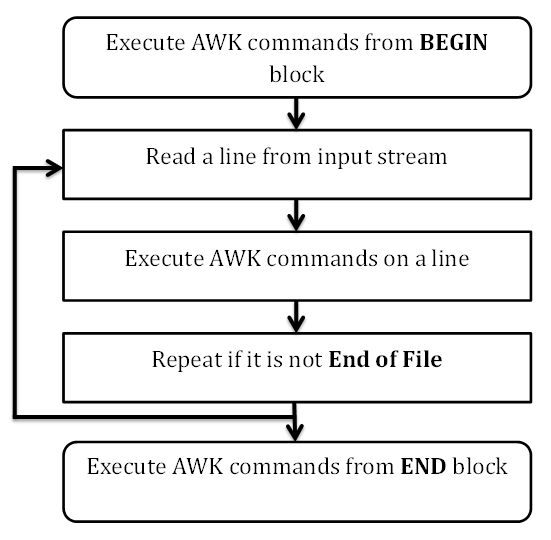
\includegraphics[width=0.4\columnwidth]{awk_workflow}
	\end{center}
	\caption{Awk Workflow}
        \label{fig:shapes}
\end{figure*}
    \begin{enumerate}
        \item
            Printing columns:
                \begin{lstlisting}[style=BashInputStyle]
                     awk '/a/ {print $3 "\t" $4}' marks.txt 
                \end{lstlisting}
        \item
            Adding variables:
                \begin{lstlisting}[style=BashInputStyle]
                     awk '/a/{++cnt} END {print "Count=", cnt}' marks.txt
                \end{lstlisting}
  \end{enumerate}
\section{Latex}
	\LaTeX is a typesetting system that is very suitable for producing scientific and mathematical documents of high typographical quality. It is also suitable for producing all sorts of other documents, from simple letters to complete books.\\
	\\
	\LaTeX enables authors to typeset and print their work at the highest typographical quality, using a predefined, professional layout. \LaTeX was originally written by Leslie Lamport.\\
	
	\LaTeX commands are case sensitive, and take one of the following two formats:
	\begin{enumerate}
		\item They start with a backslash \textbackslash and then have a name consisting of
		letters only. Command names are terminated by a space, a number or
		any other 'non-letter.'
		\item They consist of a backslash and exactly one non-letter.
		\item Many commands exist in a 'starred variant' where a star is appended
		to the command name.
	\end{enumerate}
\subsection{Input File Structure}
	When \LaTeX processes an input file, it expects it to follow a certain structure. Thus every input file must start with the command.
	\begin{verbatim}
		\documentclass{...}
	\end{verbatim}

This specifies what sort of document you intend to write. After that, add commands to influence the style of the whole document, or load packages that add new features to the \LaTeX system. To load such a package you use the command.	\\
	\begin{verbatim}
		\usepackage{...}
	\end{verbatim}
When all the setup work is done, you start the body of the text with the command.
	\begin{verbatim}
		\begin{docu\section{Latex}
	\LaTeX is a typesetting system that is very suitable for producing scientific and mathematical documents of high typographical quality. It is also suitable for producing all sorts of other documents, from simple letters to complete books.\\
	\\
	\LaTeX enables authors to typeset and print their work at the highest typographical quality, using a predefined, professional layout. \LaTeX was originally written by Leslie Lamport.\\
	
	\LaTeX commands are case sensitive, and take one of the following two formats:
	\begin{enumerate}
		\item They start with a backslash \textbackslash and then have a name consisting of
		letters only. Command names are terminated by a space, a number or
		any other 'non-letter.'
		\item They consist of a backslash and exactly one non-letter.
		\item Many commands exist in a 'starred variant' where a star is appended
		to the command name.
	\end{enumerate}
	\subsection{Input File Structure}
	When \LaTeX processes an input file, it expects it to follow a certain structure. Thus every input file must start with the command.
	\begin{verbatim}
		\documentclass{...}
	\end{verbatim}

This specifies what sort of document you intend to write. After that, add commands to influence the style of the whole document, or load packages that add new features to the \LaTeX system. To load such a package you use the command.	\\
	\begin{verbatim}
		\usepackament}
	\end{verbatim}
	Now you enter the text mixed with some useful \LaTeX commands. At the end of the document you add the
	\begin{verbatim}
	\end{document}
	\end{verbatim}
	\subsection{Titles, Chapters, and Sections}
	To help the reader find his or her way through your work, you should divide it into chapters, sections, and subsections. \LaTeX supports this with special commands that take the section title as their argument. It is up to you to use them in the correct order.\\
	The following sectioning commands are available for the \textbf{article} class:
	\begin{verbatim}
	\section{...}
	\subsection{...}
	\subsubsection{...}
	\paragraph{...}
	\subparagraph{...}
	\end{verbatim}
	If you want to split your document into parts without influencing the section or chapter numbering use:
	\begin{verbatim}
		\part{...}
	\end{verbatim}
	\LaTeX creates a table of contents by taking the section headings and page
	numbers from the last compile cycle of the document. The command
	\begin{verbatim}
		\tableofcontents
	\end{verbatim}
	The title of the whole document is generated by issuing a command:
	\begin{verbatim}
		\maketitle
	\end{verbatim}
	a footnote is printed at the foot of the current page. Footnotes should always
	be put after the word or sentence they refer to. Footnotes referring to a
	sentence or part of it should therefore be put after the comma or period.
	\begin{verbatim}
	\footnote{footnote text}
	\end{verbatim}
	In scientific publications it is customary to start with an abstract which gives
	the reader a quick overview of what to expect. \LaTeX provides the \textbf{abstract}
	environment for this purpose. Normally \textbf{abstract} is used in documents
	typeset with the article document clas
	\begin{verbatim}
		\begin{abstract}
			The abstract abstract.
		\end{abstract}
	\end{verbatim}
	
\subsection{Tables}
The tabular environment can be used to typeset beautiful tables with
optional horizontal and vertical lines. \LaTeX determines the width of the
columns automatically.\\

Below you can see the simplest working example of a table :

\begin{verbatim}

\begin{center}
\begin{tabular}{ c c c }
cell1 & cell2 & cell3 \\ 
cell4 & cell5 & cell6 \\  
cell7 & cell8 & cell9    
\end{tabular}
\end{center}

\end{verbatim}

\begin{verbatim}
	cell1  cell2  cell3
	cell4  cell5  cell6
	cell7  cell8  cell9
\end{verbatim}
\begin{verbatim}
The tabular environment is more flexible, you can put separator lines in between each column.\\
\end{verbatim}

It was already said that the tabular environment is used to type tables. To be more clear about how it works below is a description of each command.
\begin{verbatim}
{ |c|c|c| }
\end{verbatim}
This declares that three columns, separated by a vertical line, are going to be used in the table. Each c means that the contents of the column will be centred, you can also use r to align the text to the right and l for left alignment. 
\begin{verbatim}
	\hline
\end{verbatim}

This will insert a horizontal line on top of the table and at the bottom too. There is no restriction on the number of times you can use \begin{verbatim}
\hline
\end{verbatim}
. 
\begin{verbatim}
cell1 & cell2 & cell3 \\
Each & is a cell separator and the double-backslash \\ sets the end of this row. 
\end{verbatim}
\subsection{Typesetting Mathematical Formulae}
A mathematical formula can be typeset in-line within a paragraph (text style),
or the paragraph can be broken and the formula typeset separately (display
style). Mathematical equations within a paragraph are entered between \$
and \$:\\

Let's see an example of the \textbf{inline} mode: 

\begin{verbatim}
	In physics, the mass-energy equivalence is stated by the equation $E=mc^2$,
	discovered in 1905 by Albert Einstein.
\end{verbatim}

The displayed mode has two versions: numbered and unnumbered.\\
\begin{verbatim}
The mass-energy equivalence is described by the famous equation

$$E=mc^2$$

discovered in 1905 by Albert Einstein. 
In natural units ($c$ = 1), the formula expresses the identity

\begin{equation}
E=m
\end{equation}
\end{verbatim}


The \textit{amsmath} package provides a handful of options for displaying equations. You can choose the layout that better suits your document, even if the equations are really long, or if you have to include several equations in the same line.
    \section{Octave}
GNU Octave is software featuring a high-level programming language, primarily intended for numerical computations. It provides a command-line interface for solving linear and nonlinear problems numerically, and for performing other numerical experiments using a language that is mostly compatible with MATLAB. It may also be used as a batch-oriented language. It is part of the GNU Project, it is free software under the terms of the GNU General Public License.

Octave is one of the major free alternatives to MATLAB, others being Julia and Scilab. These however put less emphasis on (bidirectional) syntactic compatibility with MATLAB than Octave does.
        \subsection{MATLAB compatibility}
Octave has been built with MATLAB compatibility in mind, and shares many features with MATLAB:
            \begin{enumerate}
                    \item
                        Matrices as fundamental data type.
                    \item
                        Built-in support for complex numbers.
                    \item
                        Powerful built-in math functions and extensive function libraries.
                    \item
                        Extensibility in the form of user-defined functions.
            \end{enumerate}
            Due to this, it is easy to look for octave's documentation on Mathworks at \url{http://in.mathworks.com/}

\section{gnuplot}
		\textbf{Gnuplot} is a portable command-line driven graphing utility for Linux, OS/2, MS Windows, OSX, VMS, and many other platforms. The source code is copyrighted but freely distributed (i.e., you don't have to pay for it). It was originally created to allow scientists and students to visualize mathematical functions and data interactively, but has grown to support many non-interactive uses such as web scripting. It is also used as a plotting engine by third-party applications like Octave. Gnuplot has been supported and under active development since 1986. \\
		
		A simple example which plots the the three graphs mentioned on the same co-ordinate system:
		\begin{verbatim}
			set title "Some math functions"
			set xrange [-10:10]
			set yrange [-2:2]
			set zeroaxis
			plot (x/4)**2, sin(x), 1/x
			
		\end{verbatim}
		The supported functions include: 
		\begin{center}
			\begin{tabular}{ c c }
			      abs(x)      &      absolute value of x, $|x|$\\
			      acos(x)     &    arc-cosine  of x\\
			      asin(x)     &      arc-sine    of x\\  
			      atan(x)     &      arc-tangent of x\\
			      cos(x)      &      cosine      of x,  x is in radians.\\
			      cosh(x)     &      hyperbolic cosine of x, x is in radians\\
			      erf(x)      &      error function of x\\
			      exp(x)      &      exponential function of x, base e\\
			      inverf(x)   &      inverse error function of x\\
			      invnorm(x)  &      inverse normal distribution of x\\
			      log(x)      &      log of x, base e\\
			      log10(x)    &      log of x, base 10\\
			      norm(x)     &      normal Gaussian distribution function\\
			      rand(x)     &      pseudo-random number generator      \\
			      sgn(x)      &      1 if $x > 0$, -1 if $x < 0$, 0 if $x=0$\\
			      sin(x)      &      sine      of x, x is in radians\\
			      sinh(x)     &      hyperbolic sine of x, x is in radians\\
			      sqrt(x)     &      the square root of x\\
			      tan(x)      &      tangent of x, x is in radians\\
			      tanh(x)     &      hyperbolic tangent of x, x is in radians  
			    \end{tabular}
			\end{center}
\subsection{GNUPLOT SCRIPTS }  
Sometimes, several commands are typed to create a particular plot, and it is easy to make a typographical error when entering a command. To stream- line your plotting operations, several Gnuplot commands may be combined into a single script file. For example, the following file will create a customized display of the force-deflection data:
	 
	 \begin{verbatim}
	       # Gnuplot script file for plotting data in file "force.dat"
	       # This file is called   force.p
	       set   autoscale                        # scale axes automatically
	       unset log                              # remove any log-scaling
	       unset label                            # remove any previous labels
	       set xtic auto                          # set xtics automatically
	       set ytic auto                          # set ytics automatically
	       set title "Force Deflection Data for a Beam and a Column"
	       set xlabel "Deflection (meters)"
	       set ylabel "Force (kN)"
	       set key 0.01,100
	       set label "Yield Point" at 0.003,260
	       set arrow from 0.0028,250 to 0.003,280
	       set xr [0.0:0.022]
	       set yr [0:325]
	       plot    "force.dat" using 1:2 title 'Column' with linespoints , \
	       "force.dat" using 1:3 title 'Beam' with points
	 \end{verbatim}
	 
	 \subsection{CUSTOMIZING YOUR PLOT }
	 Many items may be customized on the plot, such as the ranges of the axes, the labels of the x and y axes, the style of data point, the style of the lines connecting the data points, and the title of the entire plot. 
	 \subsubsection{plot command customization }
	  Plots may be displayed in one of eight styles: lines, points, linespoints, impulses, dots, steps, fsteps, histeps, errorbars, xerrorbars, yerrorbars, xyerrorbars, boxes, boxerrorbars, boxxyerrorbars, financebars, candlesticks or vector To specify the line/point style use the plot command as follows: \\
	  \begin{verbatim}
	        gnuplot> plot "force.dat" using 1:2 title 'Column' with lines, \
	        "force.dat" u 1:3 t 'Beam' w linespoints
	  \end{verbatim}
	  Note that the words: using , title , and with can be abbreviated as: u, t, and w. Also, each line and point style has an associated number. 
	  \subsubsection{ set command customization}
	   Customization of the axis ranges, axis labels, and plot title, as well as many other features, are specified using the set command. Specific examples of the set command follow. (The numerical values used in these examples are arbitrary.) To view your changes type: replot at the gnuplot$>$ prompt at any time. 
	   \begin{verbatim}
	         Create a title:                  > set title "Force-Deflection Data" 
	         Put a label on the x-axis:       > set xlabel "Deflection (meters)"
	         Put a label on the y-axis:       > set ylabel "Force (kN)"
	         Change the x-axis range:         > set xrange [0.001:0.005]
	         Change the y-axis range:         > set yrange [20:500]
	         Have Gnuplot determine ranges:   > set autoscale
	         Move the key:                    > set key 0.01,100
	         Delete the key:                  > unset key
	         Put a label on the plot:         > set label "yield point" at 0.003, 260 
	         Remove all labels:               > unset label
	         Plot using log-axes:             > set logscale
	         Plot using log-axes on y-axis:   > unset logscale; set logscale y 
	         Change the tic-marks:            > set xtics (0.002,0.004,0.006,0.008)
	         Return to the default tics:      > unset xtics; set xtics auto
	         
	         
	   \end{verbatim}
\section{XFig}
Xfig  is a menu-driven tool that allows the user to draw and manipulate
objects interactively under the X Window System.  \emph{ It runs under X
version  } and requires a two- or three-button mouse.
file specifies the name of a file to be edited.   The  objects  in  the
file will be read at the start of xfig.
\\
The figure generated by xfig needs to be post processed by an external tool
to convert to a different, more usable format like JPEG or PNG. This is
usually done with \emph{fig2dev}, a program found in the Transfig package.
\\
XFig was one of the first widely used vector graphics editor (in contrast,
programs like photoshop use raster graphics), which means the images are
essentially stored in forms of bazie curves, basic shapes and straight lines
instead of having separate colors for different pixels. Due to the advent
of other programs like Inkscape which used a lot more of today's available
hardware, the program XFig now belongs as a part of history and is no longer
as popular as it used to be.

\subsection{Drawing Tools}
Most of the drawing tool operations are straight forward, but here are
some miscellaneous hints on the use of the various tools:
\begin{enumerate}
    \item The Spline Curves are the only available method for constructing
        smooth curves.  The upper spline passes through the two end points and approximates
        the other entered points.  The lower spline passes through all the drawn points
    \item The Line is drawn by specifying the starting point and subsequent points
        with mouse button 1 and the end point with mouse button 2.  A freehand line (and
        spline) may be drawn by starting with mouse button 2.
    \item When the Regular Polygon tool is selected, a parameter box appears at
        the bottom of the screen, allowing one to specify the number of vertices in the
        polygon.  By creating a polygon with n vertices and then drawing construction
        lines from the centre of the polygon to the vertices, one can subdivide a circle
        into n-1 equal segments.  This is useful when drawing something like a Compass
        Rose, for example.
    \item The Arc is specified by marking three points with mouse button 1.  When a
        precise arc is required, it is often useful to first draw a circle with the
        desired radius and centre point.  Then place the arc points on the circumference
        of the circle as required, and erase the circle
\end{enumerate}

\subsection{Grouping}
One of the most useful functions in any drawing program is the ability to specify a
group of symbols into what is called a compound object.  This effectively allows
you to create any object and then move it as a unit in the drawing.

\subsection{Scaling}
The scaling control is quite versatile: an object may be scaled horizontally,
vertically or diagonally.  The last method changes the size of the object without
changing its proportions.

\subsection{Align}
This tool is useful when you want a precise alignment, vertical or horizontal,
and snap-to-grid is not an option.
\begin{enumerate}
    \item Group the objects to be aligned
    \item Select the Align tool
    \item From the Alignment Parameters at the bottom of the drawing area,
        select the type of alignment desired (one of six possiblities)
    \item Click on the group and the objects in it will be aligned as required.
\end{enumerate}

\subsection{Update Parameter}
This tool is not a must-use when you are first learning XFig, but it can be a real
time-saver later.  The Update tool allows you to change an object’s properties by
clicking on the object.  As a consequence, it is especially useful when a large
number of objects must be changed.  For example, you might decide that every text
string on a drawing should be larger .  One possible technique is to Edit every
text string.  However , Update is much faster .  Here’s how it works:
When you select the Update function, the Update Parameters are shown at the
bottom of the screen.  Unfortunately, there’s not enough room to show them all, but
the important ones are there.  (You may have to scroll it using the scrollbar
below it to see all the parameters).  Now, when you click on an object, its
properties will be changed to the properties sho wn in the Update Parameters list.

\subsection{Incorporating Figures in Text}
XFig includes an Export facility , in which the file description may be exported
to different file formats.  The most useful ones are Latex Picture, Pictex,
Postscript , Encapsulated Postscript and bitmap formats such as GIF, JPEG
, TIFF and several others.  The different file formats allow figures, drawn in XFig
to be read by other computer programs and incorporated in various text documents.

\subsubsection{\LaTeX{} Picture Format}
The \LaTeX{}  text processing language has a limited number of drawing commands: circle,
box, and line, and these may be used to draw simple pictures.  For the Latex Picture
format, XFig copies out a description of the picture in commands that can be directly
processed by \LaTeX.  The file may be called into the main text document with the
\LaTeX{} commands.
\subsubsection{Pictex Format}
There are certain drawing elements that \LaTeX{} cannot cope with directly.  For
example, lines at certain slopes, circles of certain diameter , and continuous spline
curves are not allowed.  To cope with this, the Pictex format does all drawing by
placing a series of points.  As a result, the the Pictex format can describe extremely
complex images, but there is a price to pay .  The Pictex format is both larger and
slower to process (much slower) than the Latex format.  A document with many Pictex
inclusions can bring a 486-66 to its knees, so it is best to use Pictex only when needed.
\newpage
\section{Git}
\subsection{Introduction}
A \textbf{version control system (VCS)} allows you to track the history of a collection of files. It supports creating different versions of this collection. Each version captures a snapshot of the files at a certain point in time and the VCS allows you to switch between these versions. These versions are stored in a specific place, typically called a repository.
\textbf{Git} is a widely used source code management system for software development. It is a \textbf{distributed revision control system} with an emphasis on speed, data integrity, and support for distributed, non-linear workflows. In a distributed version control system each user has a complete local copy of a repository on his individual computer. The user can copy an existing repository. This copying process is typically called cloning and the resulting repository can be referred to as a clone.
    
    \subsection{Git terminology}
    \begin{itemize}
        \item \textbf{Cloning} : The process of copying an existing Git repository is called cloning. After cloning a repository the user has the complete repository with its history on his local machine. 
        \item \textbf{Working Tree} : A local repository provides at least one collection of files which originate from a certain version of the repository. This collection of files is called the working tree.
        \item \textbf{Branching} : Git supports branching which means that you can work on different versions of your collection of files. A branch separates these different versions and allows the user to switch between these versions to work on them.
        \item \textbf{Repository} : A repository contains the history, the different versions over time and all different branches and tags. In Git each copy of the repository is a complete repository.
        \item \textbf{Commit} : When you commit your changes into a repository this creates a new commit object in the Git repository. This commit object uniquely identifies a new revision of the content of the repository.
    \end{itemize}
    
    \subsection{Setting up a Repository}
    \subsubsection{git init}
        The git init command creates a new Git repository. It can be used to convert an existing, unversioned project to a Git repository or initialize a new empty repository.  Executing git init creates a .git subdirectory in the project root, which contains all of the necessary metadata for the repo. 
       
        \textbf{git init}
        Transform the current directory into a Git repository. This adds a .git folder to the current directory and makes it possible to start recording revisions of the project.
        
    \subsubsection{git clone}
        The git clone command copies an existing Git repository. 
        
        \textbf{git clone "repo"}
        Clone the repository located at <repo> onto the local machine. The original repository can be located on the local filesystem or on a remote machine accessible via HTTP or SSH.
    
    \subsection{Saving changes}
    \subsubsection{git add}
        The git add command adds a change in the working directory to the staging area. It tells Git that you want to include updates to a particular file in the next commit. However, git add doesn't really affect the repository in any significant way—changes are not actually recorded until you run git commit.

        \textbf{git add "file"}
        Stage all changes in "file" for the next commit.
    
    \subsubsection{git commit}
        The git commit command commits the staged snapshot to the project history. Committed snapshots can be thought of as “safe” versions of a project—Git will never change them unless you explicity ask it to. 

        \textbf{git commit}
        Commit the staged snapshot. This will launch a text editor prompting you for a commit message. After you’ve entered a message, save the file and close the editor to create the actual commit. 

        \textbf{git commit -m "message"}
        Commit the staged snapshot, but instead of launching a text editor, use "message" as the commit message.    
    \subsection{Inspecting a repository}
    \subsubsection{git status}
        The git status command displays the state of the working directory and the staging area. It lets you see which changes have been staged, which haven’t, and which files aren’t being tracked by Git. Status output does not show you any information regarding the committed project history.

        \textbf{git status}
        List which files are staged, unstaged, and untracked.

    \subsection{Viewing old commits}
    \subsubsection{git checkout}
        The git checkout command serves three distinct functions: checking out files, checking out commits, and checking out branches. In this module, we’re only concerned with the first two configurations.

        Checking out a commit makes the entire working directory match that commit. This can be used to view an old state of your project without altering your current state in any way. Checking out a file lets you see an old version of that particular file, leaving the rest of your working directory untouched.

        \textbf{git checkout master}
            Return to the master branch. Branches are covered in depth in the next module, but for now, you can just think of this as a way to get back to the “current” state of the project.

        \textbf{git checkout "commit" "file"}
        Check out a previous version of a file. This turns the "file" that resides in the working directory into an exact copy of the one from "commit" and adds it to the staging area.

        \textbf{git checkout "commit"}
        Update all files in the working directory to match the specified commit. You can use either a commit hash or a tag as the "commit" argument.

    \subsection{Undoing Changes}
    \subsubsection{git revert}

        The git revert command undoes a committed snapshot. But, instead of removing the commit from the project history, it figures out how to undo the changes introduced by the commit and appends a new commit with the resulting content. This prevents Git from losing history.

        \textbf{git revert "commit"}
        Generate a new commit that undoes all of the changes introduced in "commit", then apply it to the current branch.

    \subsubsection{git reset}
        Git reset can be used to remove committed snapshots, although it’s more often used to undo changes in the staging area and the working directory. In either case, it should only be used to undo local changes—you should never reset snapshots that have been shared with other developers.

        \textbf{git reset "file"}
        Remove the specified file from the staging area, but leave the working directory unchanged. This unstages a file without overwriting any changes.

        \textbf{git reset}
        Reset the staging area to match the most recent commit, but leave the working directory unchanged. 

    \subsubsection{git clean}
        The git clean command removes untracked files from your working directory. This is really more of a convenience command, since it’s trivial to see which files are untracked with git status and remove them manually. Like an ordinary rm command, git clean is not undoable, so make sure you really want to delete the untracked files before you run it.

        \textbf{git clean -n}
        Perform a “dry run” of git clean. This will show you which files are going to be removed without actually doing it.

        \textbf{git clean -f}
        Remove untracked files from the current directory. The -f (force) flag is required unless the clean.requireForce configuration option is set to false (it's true by default). 


\section{BitBucket}
\subsection{Introduction}
    Bitbucket is a web-based hosting service for projects that use either the Mercurial (since launch) or Git (since October 2011) revision control systems. Bitbucket offers both commercial plans and free accounts. It offers free accounts with an unlimited number of private repositories. It is a system for hosting version control repositories owned by Atlassian. It is a competitor to github.
\subsection{Creating a Git repository}
    \begin{enumerate}
        \item From Bitbucket, click Repositories and then Create repository button at the top of the page.
         The system displays the Create a new repository page.
        \item Enter BitbucketStationLocations for the Name field.
    Bitbucket uses this Name in the URL of the repository. For example, if the user thebest has a repository called awesomerepo, the URL for that repository would be https://bitbucket.org/thebest/awesomerepo.
        \item For Access level, leave the This is a private repository box checked. A private repository is only visible to you and those you give access to. If this box is unchecked, everyone can see your repository.
        \item Pick Git for the Repository type. 
        \item Click Create repository. Bitbucket creates repository and displays its Overview page.
    \end{enumerate}

\subsection{Cloning repository}
    \begin{enumerate}
        \item First make a directory on local machine.
        \item From Bitbucket, go to BitbucketStationLocations repository.
        Click Clone. The system displays a pop-up clone dialog. By default, the clone dialog sets the protocol to HTTPS or SSH, depending on your settings. For the purposes of this tutorial, don't change your default protocol.
        \item Copy the highlighted clone command. From terminal window, paste the command copied from Bitbucket and press Return.
    \end{enumerate}

\subsection {Create a file in Bitbucket}
    \begin{enumerate}
        \item From BitbucketStationLocations repository, click Source to open the source directory
        \item From the Source page, click New file in the top right corner.
    A page for creating the new file opens. 
        \item Enter filename in the  filename  field . Then select mode from the Syntax mode list. Finally add the following  code into the text box.
        \item Click Commit. The Commit message field appears with the message: "filename" created online with Bitbucket. Click Commit under the message field.
    \end{enumerate}

\end{document}


